\section{Analysis details}\label{sec:report}
\noindent This section summarizes the simulation, calibration, optimization, and comparison steps used in this study.

\subsection{Data and Monte Carlo Samples}

\noindent This study used simulated neutron events in the ePIC backward/negative hadronic calorimeter (nHCal). No collision data were used. Geometry descriptions
were generated from a parameterized DD4hep compact XML template in which the calorimeter was modeled as a 10-layer sampling detector with a 3/3/4 longitudinal segmentation
pattern. The geometry generation and simulation workflow was run as a standalone DD4hep/DDsim study rather than inside the full ePIC software stack. This setup allowed direct control of the geometry parameterization and candidate generation while preserving the detector-response comparison needed for this relative optimization study.

\noindent The transverse detector area was fixed to $1\,\mathrm{m}\times1\,\mathrm{m}$ with $10\,\mathrm{cm}\times10\,\mathrm{cm}$ readout cells.

\begin{figure}[H]
    \centering
    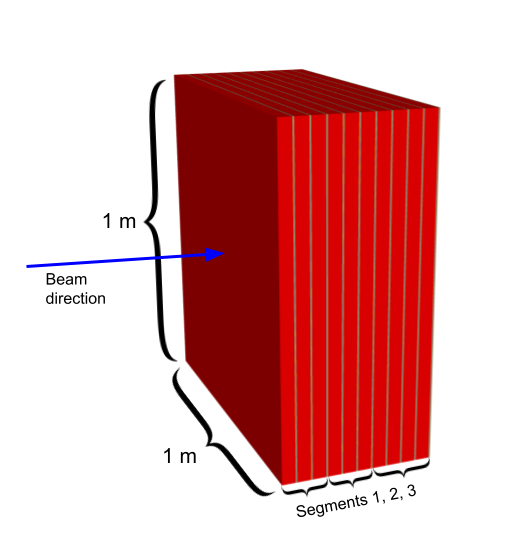
\includegraphics[width=0.55\linewidth]{plots/detector_segmentation_sketch.png}
    \caption[Detector segmentation sketch]{\it Detector sketch showing the three longitudinal segments, the absorber/scintillator parameterization, and the neutron beam direction used in the study.}
    \label{fig:nhcal_segmentation}
\end{figure}

\noindent The detector response was simulated with DD4hep/DDsim 1.36.0, Geant4 11.4.1, and ROOT 6.38.04\cite{Frank:2018dd4hep,Agostinelli:2003geant4,Allison:2006geant4,Allison:2016geant4,Brun:1997root}.
The beam configuration used a neutron G4GPS source spanning a continuous momentum range of $0.1$--$2.5~\mathrm{GeV}/c$. For neutrons, this momentum range corresponds to kinetic energies from about $5~\mathrm{MeV}$ to $1.7~\mathrm{GeV}$. Since only the lowest part of the generated spectrum lies in the range where dedicated high-precision low-energy neutron models are most relevant, the samples used the Geant4 reference physics list \texttt{FTFP\_BERT}, passed through DDsim. The source spectrum was provided as a tabulated user
histogram whose points approximate an exponential falloff, with linear interpolation between points performed by G4GPS.

\noindent The reference geometry was the uniform nHCal baseline, in which each longitudinal segment uses the same absorber and scintillator thicknesses. The nHCal is treated here as a standalone backward calorimeter element with some allowed flexibility in total depth, rather than as a geometry with a strictly fixed depth constraint. Alternative geometries
were defined by allowing the absorber and scintillator thickness to vary independently in each of the three longitudinal segments while keeping the total detector depth in a
comparable range. The initial exploration used a 150-point Latin-hypercube sample with 5000 simulated events per geometry. These values were chosen as a practical compromise
between design-space coverage and simulation cost for the first pass. Selected leading candidates were later rerun with 20000 events to reduce statistical fluctuations in the
top-ranked region while keeping the higher-stat confirmation stage computationally manageable.

\subsection{Event, Particle and PID Selections}

\noindent Only neutron gun events were used in this study. The generated momentum spectrum was fixed by the G4GPS configuration described above. No track-based reconstruction
or particle-identification selection was applied, since the study focused on calorimeter hit activity from single-particle simulation.

\noindent At the event-processing stage, an event was counted as valid if the recorded Monte Carlo energy was positive. The main performance metric, detection efficiency, was then defined as
\[
\epsilon_{\mathrm{det}}=\frac{N_{\mathrm{detected}}}{N_{\mathrm{valid}}}.
\]
An event was counted as detected if at least one calorimeter cell passed threshold anywhere in the detector. In addition to detection efficiency, two shower-activity observables
were recorded: the average number of fired tiles per valid event and the average number of fired layers per valid event. These multiplicities are treated as hit-activity observables, not standalone measures of full calorimeter performance.

\subsection{Signal Extraction}

\noindent The hit-level signal extraction was based on energy deposits in the scintillator cells. A cell was counted as fired if its deposited energy exceeded the threshold
assigned to the corresponding longitudinal segment. A layer was counted as fired if at least one cell in that layer fired.

\noindent Thresholds were derived from a MIP-based calibration step. A separate muon calibration script was used to extract a reference MIP scale from the baseline geometry.
The calibration used 10000 muon events and pooled energy deposits by layer and segment. Segment-specific thresholds for a given geometry were then obtained by linearly scaling the
reference MIP value and multiplying by the chosen MIP fraction parameter, assuming an approximately linear dependence on scintillator thickness. In the optimization runs reported here, the threshold
setting used a MIP fraction of 0.5. Figure~\ref{fig:mip_landau} shows the segment-1 baseline muon layer-energy distribution and the Landau fit used to extract the reference MPV. This thresholding procedure defines a hit-activity metric rather than a full neutron-reconstruction efficiency. This MIP-based thresholding approach follows the same general calibration logic used in internal nHCal studies\cite{Kosarzewski:2025nhcalstatus}.

\begin{figure}[H]
    \centering
    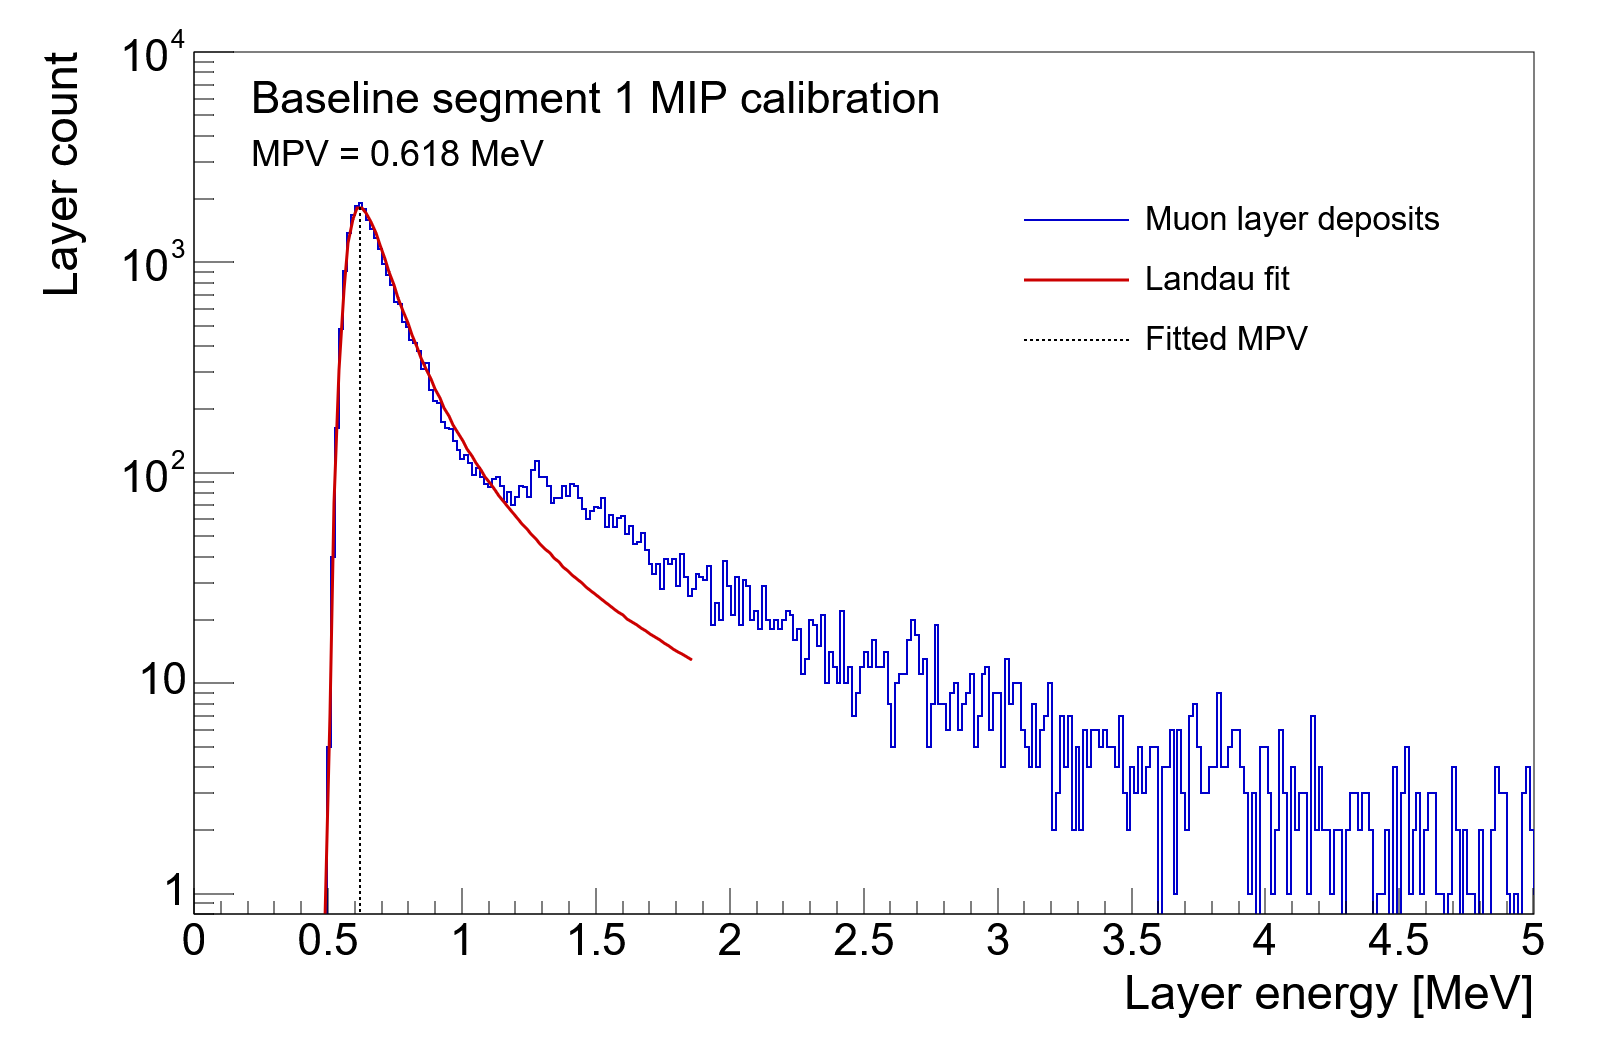
\includegraphics[width=0.72\linewidth]{plots/MIP_landau.png}
    \caption[MIP calibration distribution]{\it Muon layer-energy distribution for segment 1 of the baseline geometry. The Landau fit is restricted to the main MIP peak region and is used to extract the reference MPV for the threshold calibration.}
    \label{fig:mip_landau}
\end{figure}

\subsection{Detector-Level Corrections and Scope}

\noindent No detector-level correction procedure was applied in this study. The comparison was entirely geometry-to-geometry at the detector-response level
under a fixed simulation and thresholding workflow. The setup is relatively idealized. Because the same beam configuration, detector template, threshold definition,
and event-processing logic were used for both the baseline and all candidate geometries, the comparison is intended as a controlled relative benchmark rather than a fully corrected
absolute detector-performance measurement.

\subsection{Surrogate Model and Candidate Proposal}

\noindent The optimization stage used a surrogate-guided loop. Processed run outputs were converted into a run-level CSV and then compacted to one row per geometry. Each row
contained the absorber and scintillator thicknesses together with averaged performance metrics. The proposal loop used the composite score described below to select candidates for simulation, while the final optimum quoted in the Results section is defined by the matched neutron-efficiency comparison. The surrogate input features were:
\begin{itemize}[nosep]
    \item absorber thicknesses in segments 1, 2, and 3, each bounded to $3.5$--$4.5~\mathrm{cm}$
    \item scintillator thicknesses in segments 1, 2, and 3, each bounded to $0.3$--$0.6~\mathrm{cm}$
\end{itemize}
Together, these six geometry parameters define the design space explored in this study. The target variables were:
\begin{itemize}[nosep]
    \item neutron detection efficiency
    \item average fired-tile count
    \item average fired-layer count
\end{itemize}

\noindent The regression model was implemented with LightGBM\cite{Ke:2017lightgbm}. Because multiple target observables were predicted simultaneously, the code wrapped the base LightGBM regressor in a
multi-output regression interface. The current configuration used 500 estimators, a learning rate of 0.05, 31 leaves, and 0.8 subsampling in both rows and features. By default,
20\% of the compact dataset was held out for validation, and mean absolute percentage error was printed separately for each predicted target, consistently within 2\% for each target. These
hyperparameters were fixed settings and were not separately tuned in this study.

\noindent The surrogate ranking used a normalized weighted score built from predicted neutron detection efficiency, average fired-layer count, and average fired-tile count, with weights of
0.5, 0.3, and 0.2, respectively. For each metric, the normalization used the baseline geometry as the zero-point anchor and the 90th percentile of the initial Latin-hypercube sample
as the reference scale. Values below baseline received no credit. Values between the baseline and the 90th percentile were scaled linearly. Values above the 90th percentile were allowed
to continue increasing with a reduced slope of 0.2, so that the top end of the score did not saturate immediately while still remaining less sensitive to extreme fluctuations.

\noindent These weights prioritized neutron detection efficiency as the primary objective, while the larger secondary weight on fired-layer multiplicity gave extra preference to longitudinal shower
development in a study focused on longitudinal segmentation. The smaller fired-tile weight was retained as a weaker measure of overall shower activity. The 90th-percentile anchor was used
to reduce sensitivity to the noisiest upper tail of the initial scan.

\noindent Candidate generation for later iterations was handled by quasi-random sampling in the allowed design space. The active workflow sampled a pool of 20000 candidates per
iteration and generated 5 proposed geometries per surrogate-guided proposal batch. Design constraints were applied first in geometry space, after which the sampled candidates were converted into surrogate
feature rows and scored with the trained model. Candidate selection within a proposal batch also enforced a minimum normalized geometry-space separation of 0.05 between chosen proposals as a
practical diversity setting. The pool size and the batch size were chosen as a practical balance between broad surrogate-guided exploration and downstream simulation throughput.

\noindent After each sweep was simulated and processed, the compacted outputs were appended to the previous compact CSV and used to retrain the surrogate model. The updated model
was then used to generate the next proposed sweep. In parallel with this loop, the compact CSV was rescored directly to identify the current best observed geometry under the same objective
used for candidate ranking.

\subsection{Systematic Uncertainties}

\noindent This note did not perform a full detector-systematics study. The dominant uncertainty considered here was Monte Carlo statistical variation between geometry evaluations.
This mattered because the efficiency landscape across the scanned geometries was shallow. In the initial 150-point scan, neutron detection efficiencies covered only
a narrow range, approximately 0.51 to 0.55. This overall efficiency scale is broadly consistent with nHCal performance estimates\cite{BrandenburgRiedl:2025nhcalpdr}. Under those conditions, low-statistics
evaluations can mis-rank near-top candidates even when the broader landscape is still identified correctly.

\noindent To address this, the study used a staged event-count strategy. The initial Latin-hypercube scan used 5000 events per geometry to map the design space at manageable cost.
Top-performing candidates were then rerun with 20000 events to test whether their apparent advantage persisted at higher statistics. Several geometries that looked competitive in
the lower-stat scan did not remain leaders after these higher-stat confirmation runs. This behavior indicates that the initial low-statistics scan was useful for identifying the relevant performance region, but not sufficient by itself to rank near-tied leading candidates reliably. Because the final optimum was selected from a larger scan, the repeated-run comparison should be read as validation of a selected candidate rather than an unbiased estimate of the best possible geometry in the full design space.

\noindent For the final baseline-versus-optimum comparison, both the baseline geometry and the optimum were evaluated with ten 5000-event runs each. This provides matched repeated-run
estimates for the main observables and their standard errors on the mean. The number of repeated runs was chosen as a computationally affordable way to estimate run-to-run variation in the
final matched comparison.

\noindent A limited three-seed cross-check using the high-precision neutron physics list \texttt{FTFP\_BERT\_HP} was performed for the baseline and optimum, with 5000 events per seed. The three-seed \texttt{FTFP\_BERT\_HP} mean efficiencies were 0.5333 for the baseline and 0.5361 for the optimum, compared with 0.5317 and 0.5418 in the main \texttt{FTFP\_BERT} repeated-run comparison. The resulting efficiencies did not show a large physics-list-driven shift, but the sample was not statistically powered to resolve the small baseline--optimum separation observed in the main \texttt{FTFP\_BERT} repeated-run comparison. A broader treatment of systematic variations, such as alternative threshold settings, physics lists, or beam-shape variations, is outside the scope of the present note. The linear scaling of the MIP threshold with scintillator thickness is also treated as part of the fixed workflow and was not varied separately.


\subsection{Results}

\noindent The optimization landscape was found to be shallow. The highest-efficiency confirmed geometry was already present in the initial 150-point Latin-hypercube sample.
Later surrogate-guided proposals produced candidates with comparable performance, but they did not consistently outperform this geometry once higher-stat reruns were
used to check the leaders.

\begin{figure}[H]
    \centering
    \begin{subfigure}[t]{0.48\linewidth}
        \centering
        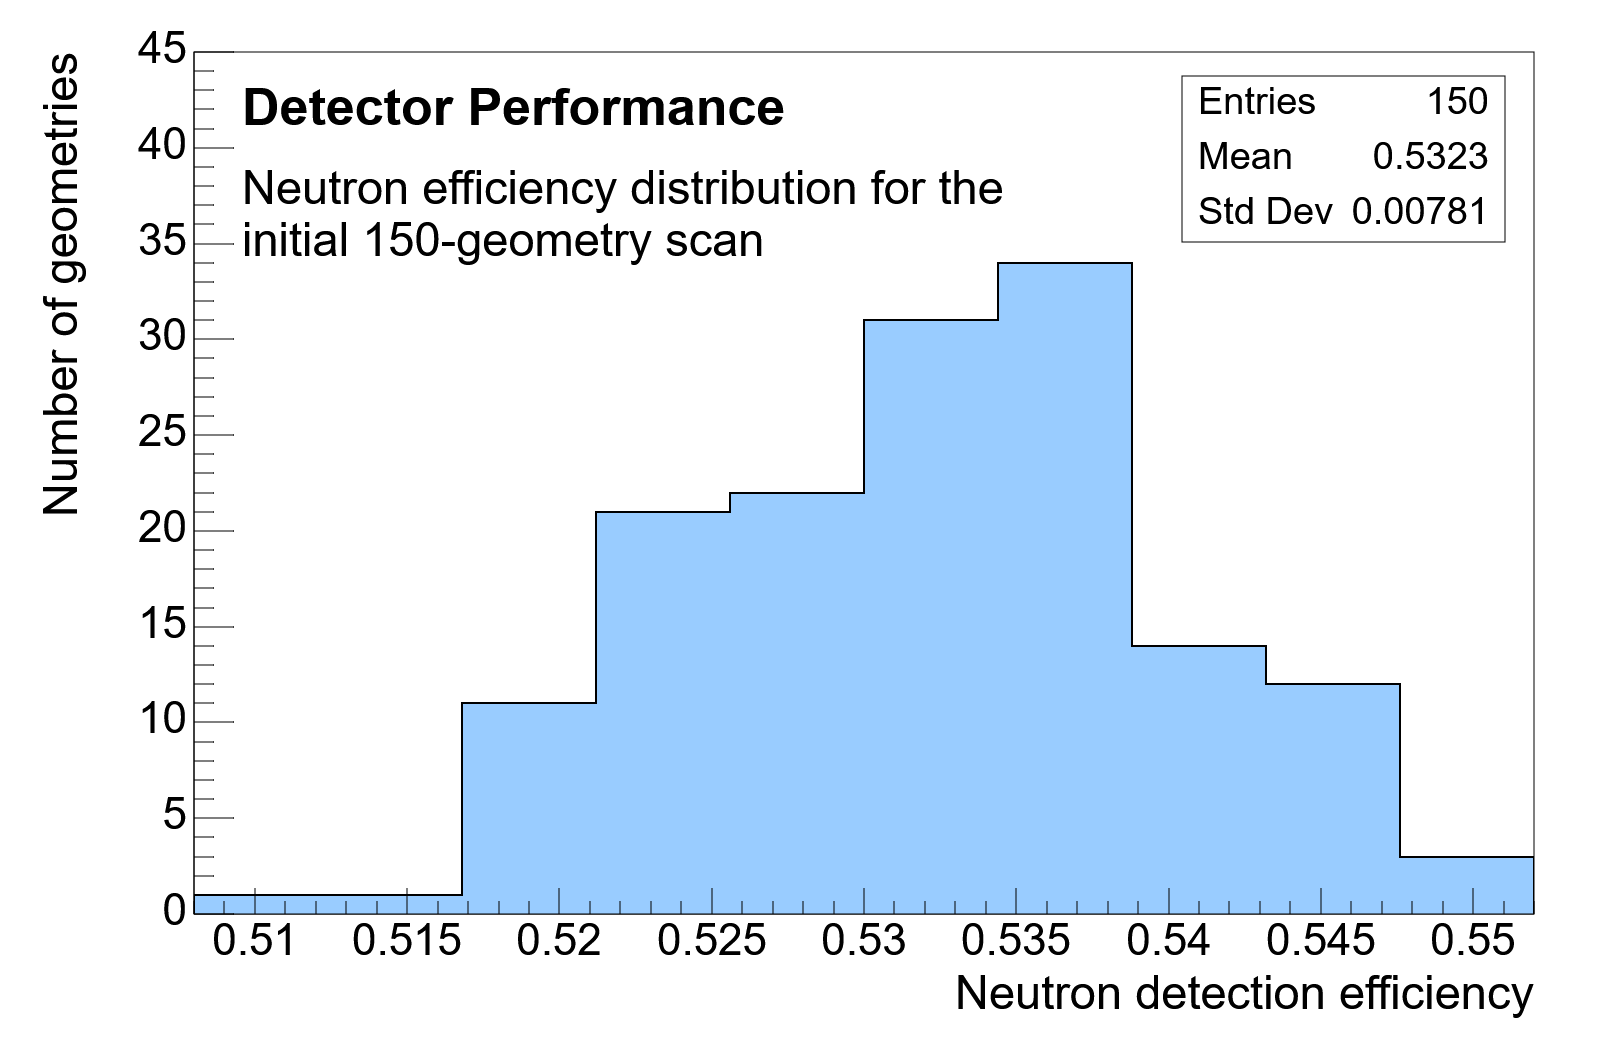
\includegraphics[width=\linewidth]{plots/efficiency_hist.png}
        \caption{\it Histogram of neutron detection efficiencies across the initial 150-geometry scan.}
        \label{fig:efficiency_histogram}
    \end{subfigure}
    \hfill
    \begin{subfigure}[t]{0.48\linewidth}
        \centering
        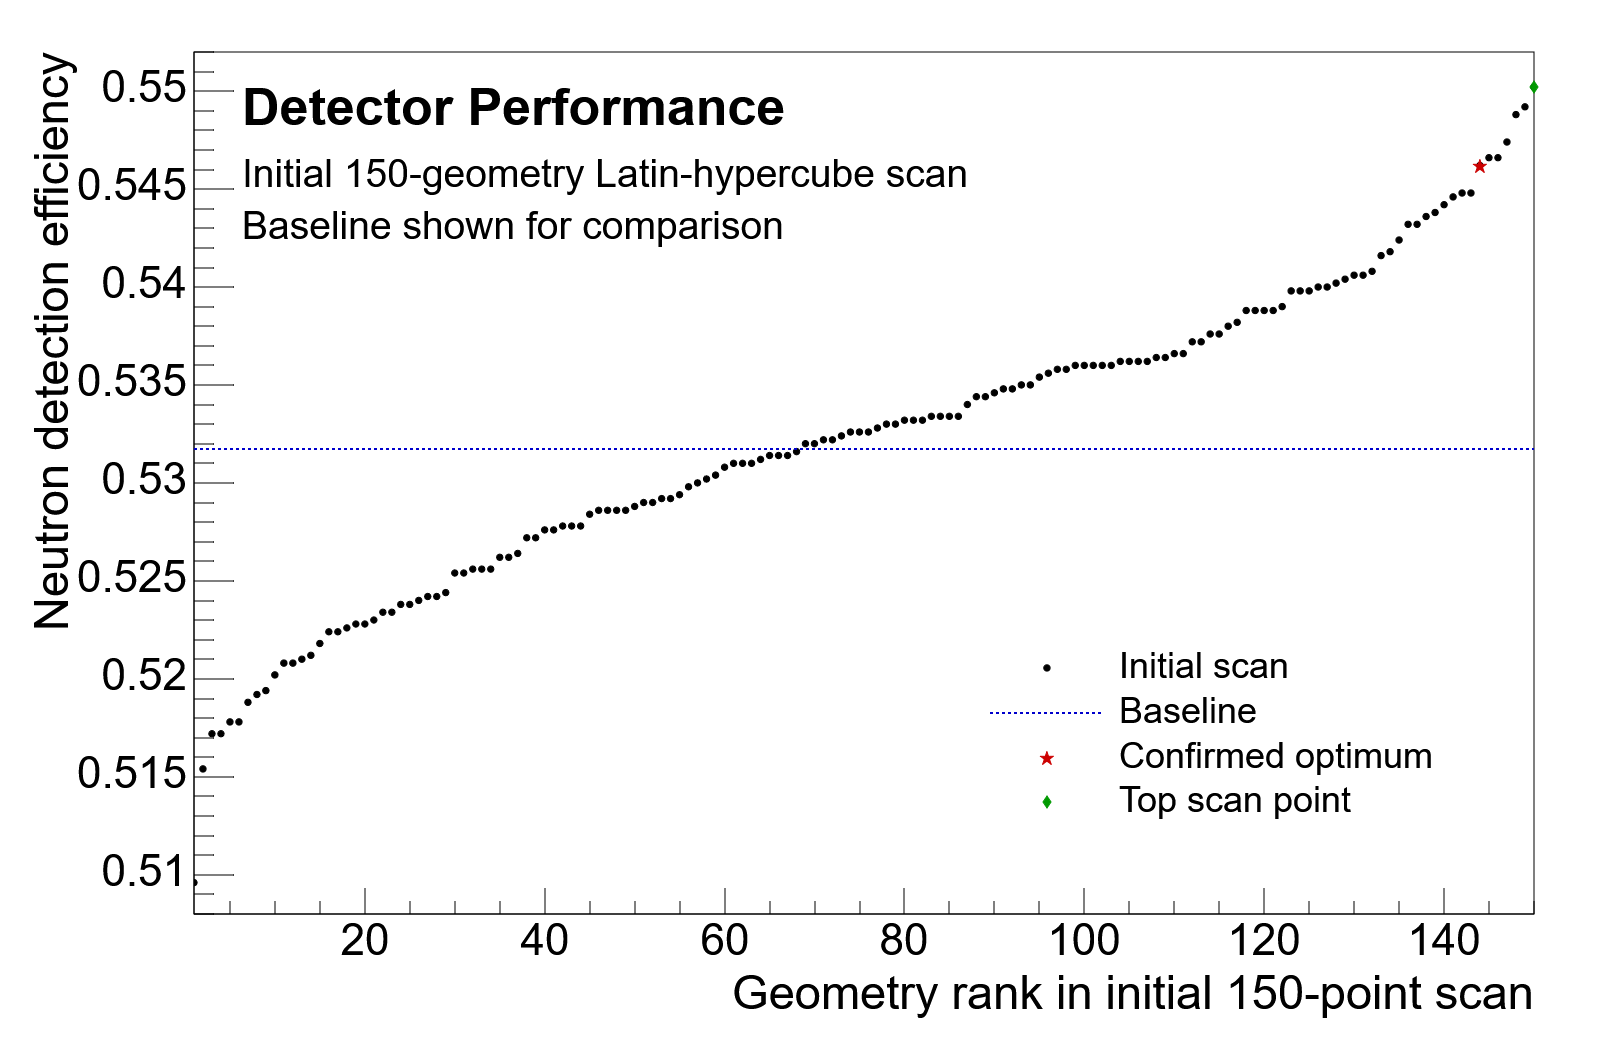
\includegraphics[width=\linewidth]{plots/sorted_efficiency.png}
        \caption{\it Sorted neutron detection efficiencies from the initial 150-geometry scan, with the baseline shown for comparison.}
        \label{fig:sorted_efficiency_scan}
    \end{subfigure}
    \caption[Efficiency landscape and sorted scan]{\it Neutron detection efficiency views for the initial 150-geometry scan.}
    \label{fig:efficiency_scan_summary}
\end{figure}

\noindent Figure~\ref{fig:efficiency_scan_summary} provides complementary views of the same shallow landscape. The left panel shows that the scanned
geometries occupy only a narrow efficiency range, while the right panel shows that many geometries remain close in performance and that the baseline lies within the broader spread of
the sampled designs.

\noindent The final matched comparison used the uniform baseline geometry and the optimum, each evaluated in ten independent 5000-event runs. The quoted uncertainties in this
paragraph are standard errors on the mean. The baseline achieved a neutron detection efficiency of $0.53172 \pm 0.00331$, while the optimum achieved $0.54184 \pm 0.00276$,
corresponding to an absolute gain of 0.01012 and a relative gain of about 2\%. Using the quoted standard errors, this efficiency difference corresponds to about 2.3 combined standard errors. Over the same comparison, the average fired-tile multiplicity increased from $1.09068 \pm 0.00897$
to $1.13452 \pm 0.00660$, and the average fired-layer multiplicity increased from $0.97710 \pm 0.00786$ to $1.01348 \pm 0.00553$. These correspond to increases of about 4.4\% and 4.1\%,
respectively.

\noindent Tables~\ref{tab:baseline_geometry}--\ref{tab:rerun_b_geometry} summarize the baseline, the optimum, and the next two best-performing geometries among the higher-stat reruns.
All thickness values are given in cm. The baseline has a total absorber depth of $40.00~\mathrm{cm}$ and a total scintillator depth of $4.00~\mathrm{cm}$, while the optimum has a total absorber depth of about $37.95~\mathrm{cm}$ and a total scintillator depth of about $4.86~\mathrm{cm}$. Using iron as an approximate proxy for the stainless-steel absorber and polystyrene for the scintillator, these correspond to about $2.44$ and $2.33$ nuclear interaction lengths for the baseline and optimum, respectively. Candidates A and B are single higher-stat comparisons and are therefore listed without repeated-run standard errors.

\begin{center}
    \begin{minipage}[t]{0.47\textwidth}
        \centering
        \begin{tabular}{lc}
            \toprule
            Metric & Value \\
            \midrule
            $t_{\mathrm{abs},1}$ & 4.0000 \\
            $t_{\mathrm{scin},1}$ & 0.4000 \\
            $t_{\mathrm{abs},2}$ & 4.0000 \\
            $t_{\mathrm{scin},2}$ & 0.4000 \\
            $t_{\mathrm{abs},3}$ & 4.0000 \\
            $t_{\mathrm{scin},3}$ & 0.4000 \\
            Efficiency & $0.53172 \pm 0.00331$ \\
            Tiles Mean & $1.09068 \pm 0.00897$ \\
            Layers Mean & $0.97710 \pm 0.00786$ \\
            \bottomrule
        \end{tabular}
        \captionof{table}[Baseline geometry]{\it Baseline geometry.}
        \label{tab:baseline_geometry}
    \end{minipage}
    \hfill
    \begin{minipage}[t]{0.47\textwidth}
        \centering
        \begin{tabular}{lc}
            \toprule
            Metric & Value \\
            \midrule
            $t_{\mathrm{abs},1}$ & 3.6138 \\
            $t_{\mathrm{scin},1}$ & 0.5121 \\
            $t_{\mathrm{abs},2}$ & 3.6732 \\
            $t_{\mathrm{scin},2}$ & 0.4663 \\
            $t_{\mathrm{abs},3}$ & 4.0268 \\
            $t_{\mathrm{scin},3}$ & 0.4801 \\
            Efficiency & $0.54184 \pm 0.00276$ \\
            Tiles Mean & $1.13452 \pm 0.00660$ \\
            Layers Mean & $1.01348 \pm 0.00553$ \\
            \bottomrule
        \end{tabular}
        \captionof{table}[Optimum geometry]{\it Optimum geometry.}
        \label{tab:optimum_geometry}
    \end{minipage}

    \vspace{0.75cm}

    \begin{minipage}[t]{0.47\textwidth}
        \centering
        \begin{tabular}{lc}
            \toprule
            Metric & Value \\
            \midrule
            $t_{\mathrm{abs},1}$ & 3.6043 \\
            $t_{\mathrm{scin},1}$ & 0.5100 \\
            $t_{\mathrm{abs},2}$ & 3.6071 \\
            $t_{\mathrm{scin},2}$ & 0.3395 \\
            $t_{\mathrm{abs},3}$ & 3.5849 \\
            $t_{\mathrm{scin},3}$ & 0.3072 \\
            Efficiency & 0.53705 \\
            Tiles Mean & 1.14130 \\
            Layers Mean & 1.02010 \\
            \bottomrule
        \end{tabular}
        \captionof{table}[High-stat candidate A]{\it First higher-stat comparison candidate.}
        \label{tab:rerun_a_geometry}
    \end{minipage}
    \hfill
    \begin{minipage}[t]{0.47\textwidth}
        \centering
        \begin{tabular}{lc}
            \toprule
            Metric & Value \\
            \midrule
            $t_{\mathrm{abs},1}$ & 3.5150 \\
            $t_{\mathrm{scin},1}$ & 0.5771 \\
            $t_{\mathrm{abs},2}$ & 3.5268 \\
            $t_{\mathrm{scin},2}$ & 0.4571 \\
            $t_{\mathrm{abs},3}$ & 4.0344 \\
            $t_{\mathrm{scin},3}$ & 0.4120 \\
            Efficiency & 0.53670 \\
            Tiles Mean & 1.14450 \\
            Layers Mean & 1.02065 \\
            \bottomrule
        \end{tabular}
        \captionof{table}[High-stat candidate B]{\it Second higher-stat comparison candidate.}
        \label{tab:rerun_b_geometry}
    \end{minipage}
\end{center}
\noindent The baseline and optimum were also compared as a function of neutron kinetic energy and MIP threshold fraction to check how the integrated result depends on the generated spectrum and hit threshold.

\begin{figure}[H]
    \centering
    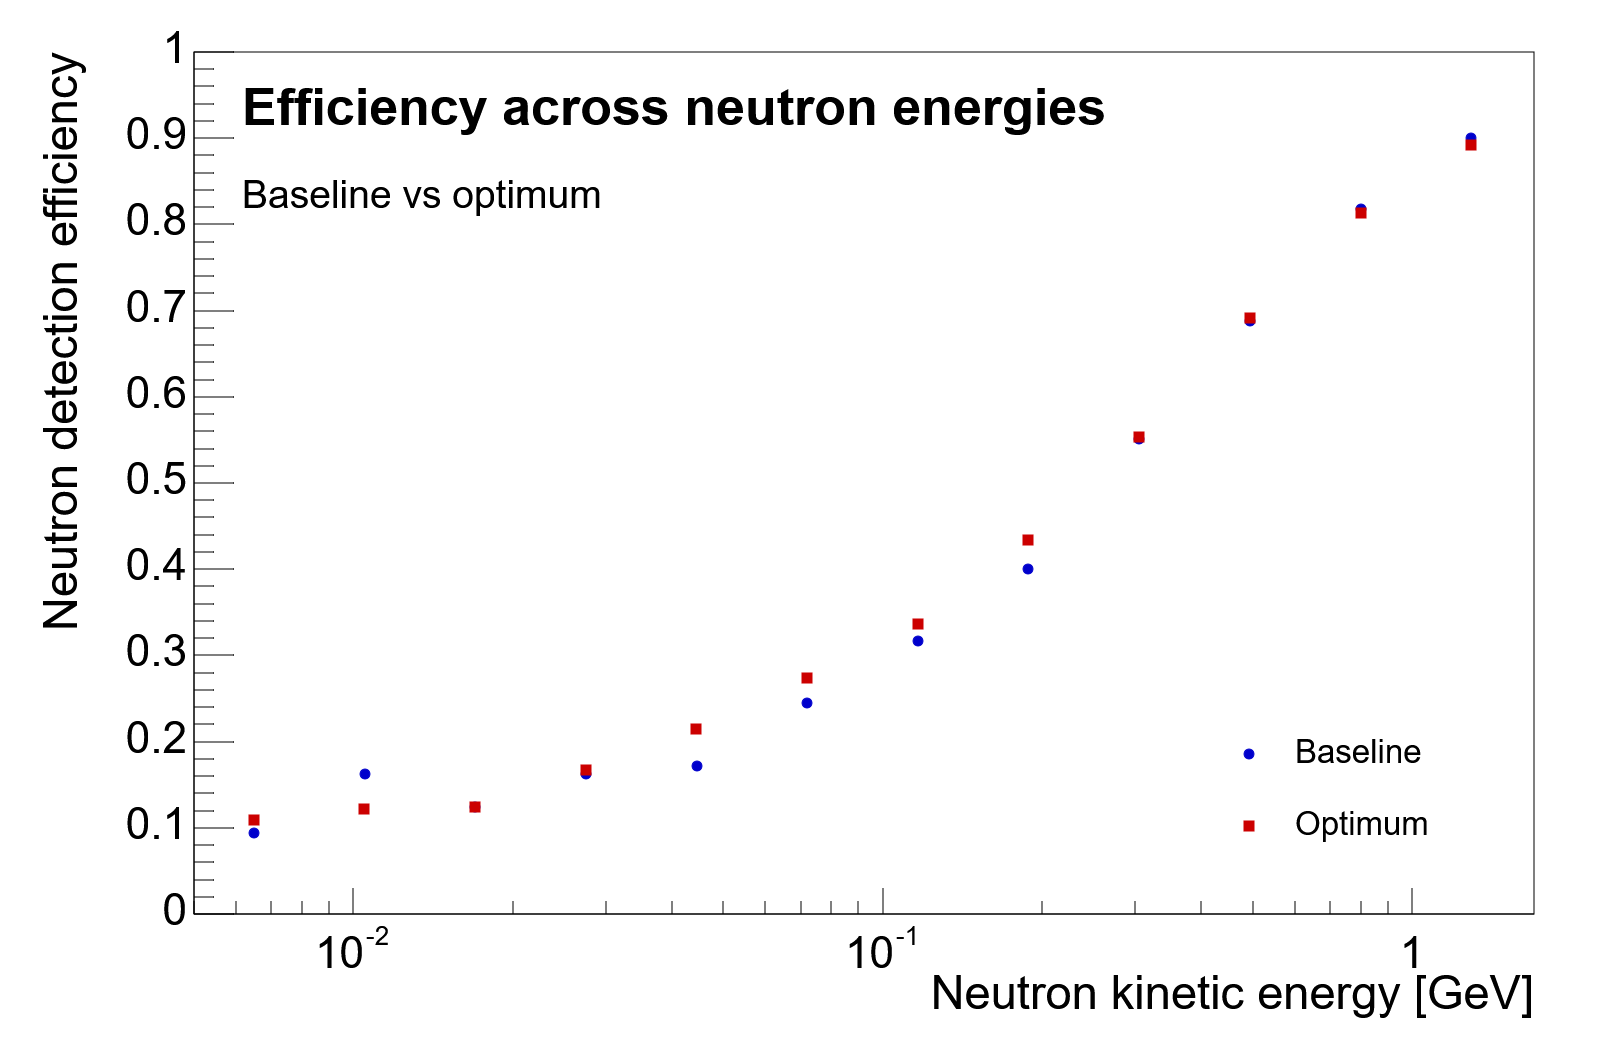
\includegraphics[width=0.72\linewidth]{plots/eff_vs_KE.png}
    \caption[Efficiency versus neutron kinetic energy]{\it Neutron detection efficiency as a function of neutron kinetic energy for the baseline and optimum geometries. The plot was produced from 20000-event samples for each geometry using the nominal 0.5-MIP threshold.}
    \label{fig:efficiency_vs_kinetic_energy}
\end{figure}

\noindent Figure~\ref{fig:efficiency_vs_kinetic_energy} shows that the detection efficiency rises with neutron kinetic energy over the generated spectrum. The largest baseline--optimum separation appears in the intermediate kinetic-energy region, roughly $0.04$--$0.19~\mathrm{GeV}$. Outside that range, the two curves remain close together, consistent with the modest integrated efficiency difference.

\begin{figure}[H]
    \centering
    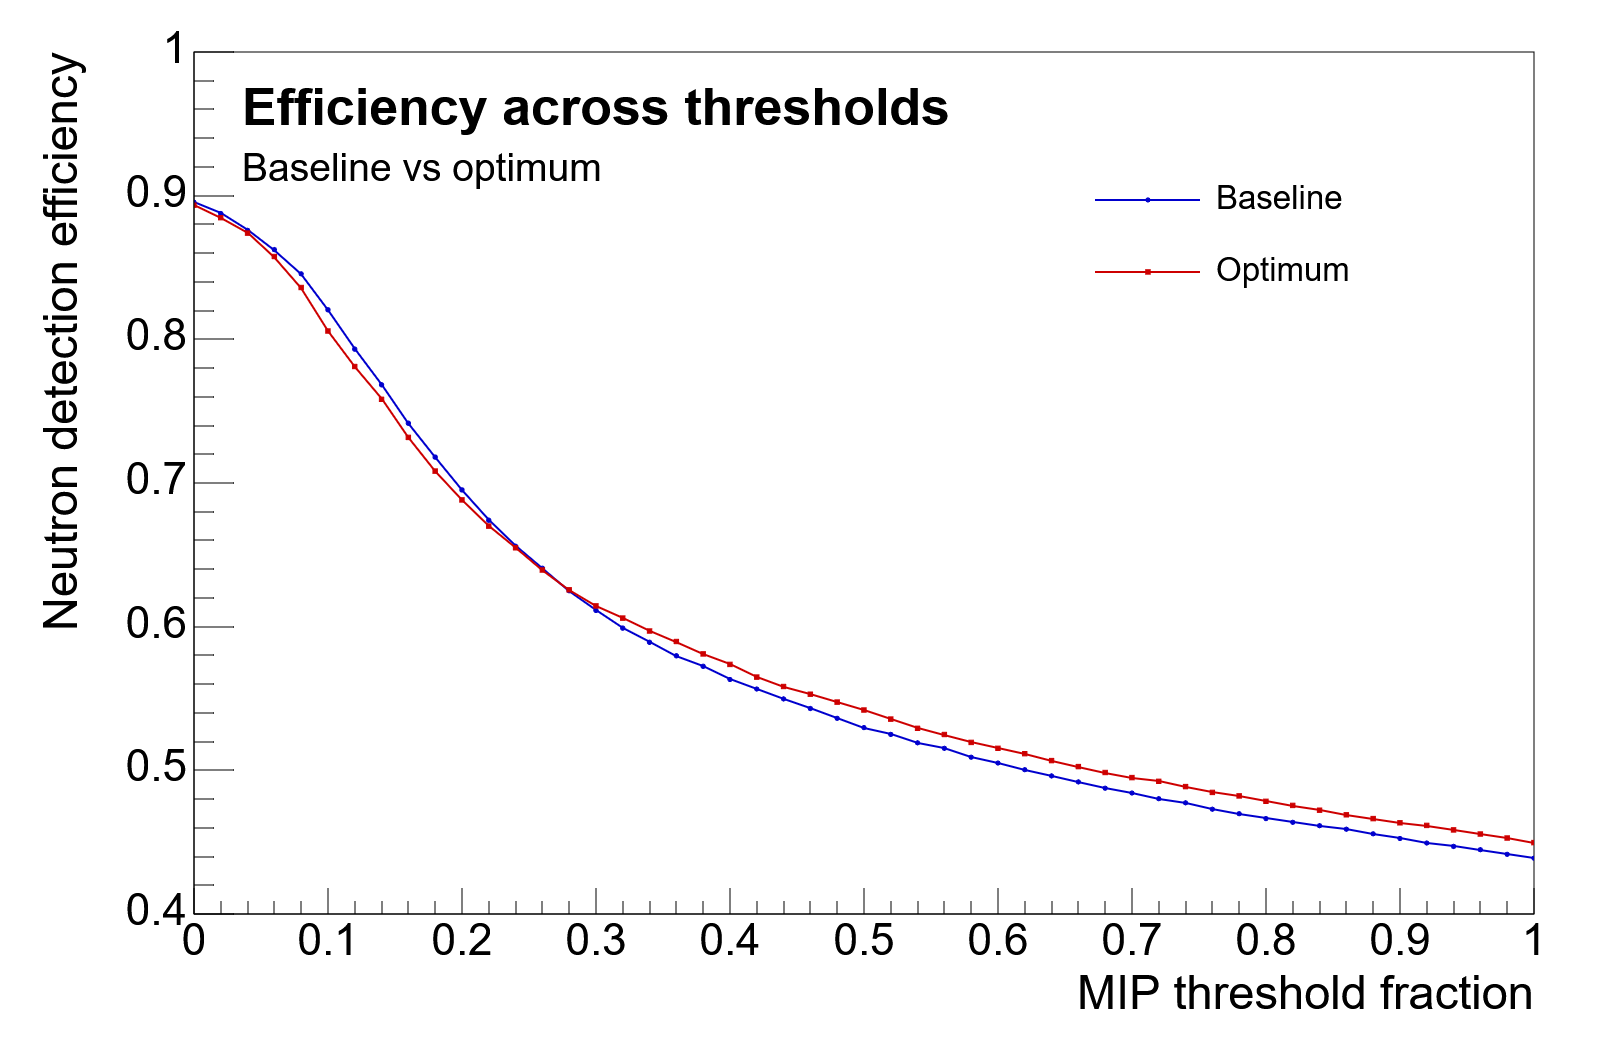
\includegraphics[width=0.72\linewidth]{plots/threshold_scan.png}
    \caption[Threshold-dependence check]{\it Threshold-dependence check for the baseline and optimum geometries. The optimum remains above the baseline near the nominal 0.5-MIP threshold and across most of the higher-threshold region, while the ordering reverses at very low threshold.}
    \label{fig:threshold_scan}
\end{figure}

\noindent The threshold scan was produced by reprocessing the same 20000-event simulated samples with different MIP threshold fractions, rather than by rerunning DDsim at each threshold. Because the same events are reused, points along each curve are correlated across threshold values. Figure~\ref{fig:threshold_scan} shows that the baseline and optimum response depends on the chosen MIP threshold fraction. At very low thresholds, below about 0.2 MIP, the baseline is comparable to or slightly above the optimum. This low-threshold region is aggressive for a binary hit-activity metric, and both geometries already have relatively high detection efficiencies there. Near the nominal 0.5-MIP operating point and across most of the higher-threshold range, the optimum remains above the baseline. The threshold scan therefore supports the nominal-threshold comparison as a feature of the operating region, while also showing that the ordering is not independent of threshold choice.

\subsection{Discussion}

\noindent The main outcome of this study is that the scanned nHCal geometry space does not show a large efficiency gradient around the baseline. The best nonuniform geometry gives a measurable but modest improvement in neutron detection efficiency, while the fired-tile and fired-layer observables show a somewhat clearer increase in shower activity. This suggests that segment-dependent longitudinal thickness variation can modestly affect the response, but the available improvement within the tested bounds is limited. Since the optimum also changes the total absorber/scintillator balance relative to the baseline, the observed gain should not be attributed uniquely to longitudinal segmentation.

\noindent The shallow landscape also explains why higher-statistics confirmation was necessary. Several geometries were close enough in performance that low-statistics simulation noise could change their apparent ordering. In this regime, the surrogate-guided workflow is used primarily to reduce the search space and identify promising regions, rather than as a standalone method for selecting a final optimum. The final baseline-versus-optimum comparison should therefore be interpreted as evidence for a small geometry-dependent effect that would benefit from further validation under larger event samples and systematic variations.
